%% bare_conf.tex
%% V1.4b
%% 2015/08/26
%% by Michael Shell
%% See:
%% http://www.michaelshell.org/
%% for current contact information.
%%
%% This is a skeleton file demonstrating the use of IEEEtran.cls
%% (requires IEEEtran.cls version 1.8b or later) with an IEEE
%% conference paper.
%%
%% Support sites:
%% http://www.michaelshell.org/tex/ieeetran/
%% http://www.ctan.org/pkg/ieeetran
%% and
%% http://www.ieee.org/

%%*************************************************************************
%% Legal Notice:
%% This code is offered as-is without any warranty either expressed or
%% implied; without even the implied warranty of MERCHANTABILITY or
%% FITNESS FOR A PARTICULAR PURPOSE! 
%% User assumes all risk.
%% In no event shall the IEEE or any contributor to this code be liable for
%% any damages or losses, including, but not limited to, incidental,
%% consequential, or any other damages, resulting from the use or misuse
%% of any information contained here.
%%
%% All comments are the opinions of their respective authors and are not
%% necessarily endorsed by the IEEE.
%%
%% This work is distributed under the LaTeX Project Public License (LPPL)
%% ( http://www.latex-project.org/ ) version 1.3, and may be freely used,
%% distributed and modified. A copy of the LPPL, version 1.3, is included
%% in the base LaTeX documentation of all distributions of LaTeX released
%% 2003/12/01 or later.
%% Retain all contribution notices and credits.
%% ** Modified files should be clearly indicated as such, including  **
%% ** renaming them and changing author support contact information. **
%%*************************************************************************


% *** Authors should verify (and, if needed, correct) their LaTeX system  ***
% *** with the testflow diagnostic prior to trusting their LaTeX platform ***
% *** with production work. The IEEE's font choices and paper sizes can   ***
% *** trigger bugs that do not appear when using other class files.       ***                          ***
% The testflow support page is at:
% http://www.michaelshell.org/tex/testflow/



\documentclass[conference]{IEEEtran}
% Some Computer Society conferences also require the compsoc mode option,
% but others use the standard conference format.
%
% If IEEEtran.cls has not been installed into the LaTeX system files,
% manually specify the path to it like:
% \documentclass[conference]{../sty/IEEEtran}





% Some very useful LaTeX packages include:
% (uncomment the ones you want to load)


% *** MISC UTILITY PACKAGES ***
%
%\usepackage{ifpdf}
% Heiko Oberdiek's ifpdf.sty is very useful if you need conditional
% compilation based on whether the output is pdf or dvi.
% usage:
% \ifpdf
%   % pdf code
% \else
%   % dvi code
% \fi
% The latest version of ifpdf.sty can be obtained from:
% http://www.ctan.org/pkg/ifpdf
% Also, note that IEEEtran.cls V1.7 and later provides a builtin
% \ifCLASSINFOpdf conditional that works the same way.
% When switching from latex to pdflatex and vice-versa, the compiler may
% have to be run twice to clear warning/error messages.






% *** CITATION PACKAGES ***
%
%\usepackage{cite}
% cite.sty was written by Donald Arseneau
% V1.6 and later of IEEEtran pre-defines the format of the cite.sty package
% \cite{} output to follow that of the IEEE. Loading the cite package will
% result in citation numbers being automatically sorted and properly
% "compressed/ranged". e.g., [1], [9], [2], [7], [5], [6] without using
% cite.sty will become [1], [2], [5]--[7], [9] using cite.sty. cite.sty's
% \cite will automatically add leading space, if needed. Use cite.sty's
% noadjust option (cite.sty V3.8 and later) if you want to turn this off
% such as if a citation ever needs to be enclosed in parenthesis.
% cite.sty is already installed on most LaTeX systems. Be sure and use
% version 5.0 (2009-03-20) and later if using hyperref.sty.
% The latest version can be obtained at:
% http://www.ctan.org/pkg/cite
% The documentation is contained in the cite.sty file itself.






% *** GRAPHICS RELATED PACKAGES ***
\usepackage{graphicx}
\usepackage{xcolor}
\usepackage{color}
\usepackage{balance}
\usepackage{booktabs}
\usepackage{multirow}
\definecolor{forestgreen}{RGB}{52,194,48}
\definecolor{truepurple}{RGB}{94, 23, 235}
%
\ifCLASSINFOpdf
  % \usepackage[pdftex]{graphicx}
  % declare the path(s) where your graphic files are
  % \graphicspath{{../pdf/}{../jpeg/}}
  % and their extensions so you won't have to specify these with
  % every instance of \includegraphics
  % \DeclareGraphicsExtensions{.pdf,.jpeg,.png}
\else
  % or other class option (dvipsone, dvipdf, if not using dvips). graphicx
  % will default to the driver specified in the system graphics.cfg if no
  % driver is specified.
  % \usepackage[dvips]{graphicx}
  % declare the path(s) where your graphic files are
  % \graphicspath{{../eps/}}
  % and their extensions so you won't have to specify these with
  % every instance of \includegraphics
  % \DeclareGraphicsExtensions{.eps}
\fi
% graphicx was written by David Carlisle and Sebastian Rahtz. It is
% required if you want graphics, photos, etc. graphicx.sty is already
% installed on most LaTeX systems. The latest version and documentation
% can be obtained at: 
% http://www.ctan.org/pkg/graphicx
% Another good source of documentation is "Using Imported Graphics in
% LaTeX2e" by Keith Reckdahl which can be found at:
% http://www.ctan.org/pkg/epslatex
%
% latex, and pdflatex in dvi mode, support graphics in encapsulated
% postscript (.eps) format. pdflatex in pdf mode supports graphics
% in .pdf, .jpeg, .png and .mps (metapost) formats. Users should ensure
% that all non-photo figures use a vector format (.eps, .pdf, .mps) and
% not a bitmapped formats (.jpeg, .png). The IEEE frowns on bitmapped formats
% which can result in "jaggedy"/blurry rendering of lines and letters as
% well as large increases in file sizes.
%
% You can find documentation about the pdfTeX application at:
% http://www.tug.org/applications/pdftex





% *** MATH PACKAGES ***
%
%\usepackage{amsmath}
% A popular package from the American Mathematical Society that provides
% many useful and powerful commands for dealing with mathematics.
%
% Note that the amsmath package sets \interdisplaylinepenalty to 10000
% thus preventing page breaks from occurring within multiline equations. Use:
%\interdisplaylinepenalty=2500
% after loading amsmath to restore such page breaks as IEEEtran.cls normally
% does. amsmath.sty is already installed on most LaTeX systems. The latest
% version and documentation can be obtained at:
% http://www.ctan.org/pkg/amsmath





% *** SPECIALIZED LIST PACKAGES ***
%
%\usepackage{algorithmic}
% algorithmic.sty was written by Peter Williams and Rogerio Brito.
% This package provides an algorithmic environment fo describing algorithms.
% You can use the algorithmic environment in-text or within a figure
% environment to provide for a floating algorithm. Do NOT use the algorithm
% floating environment provided by algorithm.sty (by the same authors) or
% algorithm2e.sty (by Christophe Fiorio) as the IEEE does not use dedicated
% algorithm float types and packages that provide these will not provide
% correct IEEE style captions. The latest version and documentation of
% algorithmic.sty can be obtained at:
% http://www.ctan.org/pkg/algorithms
% Also of interest may be the (relatively newer and more customizable)
% algorithmicx.sty package by Szasz Janos:
% http://www.ctan.org/pkg/algorithmicx




% *** ALIGNMENT PACKAGES ***
%
%\usepackage{array}
% Frank Mittelbach's and David Carlisle's array.sty patches and improves
% the standard LaTeX2e array and tabular environments to provide better
% appearance and additional user controls. As the default LaTeX2e table
% generation code is lacking to the point of almost being broken with
% respect to the quality of the end results, all users are strongly
% advised to use an enhanced (at the very least that provided by array.sty)
% set of table tools. array.sty is already installed on most systems. The
% latest version and documentation can be obtained at:
% http://www.ctan.org/pkg/array


% IEEEtran contains the IEEEeqnarray family of commands that can be used to
% generate multiline equations as well as matrices, tables, etc., of high
% quality.




% *** SUBFIGURE PACKAGES ***
%\ifCLASSOPTIONcompsoc
%  \usepackage[caption=false,font=normalsize,labelfont=sf,textfont=sf]{subfig}
%\else
%  \usepackage[caption=false,font=footnotesize]{subfig}
%\fi
% subfig.sty, written by Steven Douglas Cochran, is the modern replacement
% for subfigure.sty, the latter of which is no longer maintained and is
% incompatible with some LaTeX packages including fixltx2e. However,
% subfig.sty requires and automatically loads Axel Sommerfeldt's caption.sty
% which will override IEEEtran.cls' handling of captions and this will result
% in non-IEEE style figure/table captions. To prevent this problem, be sure
% and invoke subfig.sty's "caption=false" package option (available since
% subfig.sty version 1.3, 2005/06/28) as this is will preserve IEEEtran.cls
% handling of captions.
% Note that the Computer Society format requires a larger sans serif font
% than the serif footnote size font used in traditional IEEE formatting
% and thus the need to invoke different subfig.sty package options depending
% on whether compsoc mode has been enabled.
%
% The latest version and documentation of subfig.sty can be obtained at:
% http://www.ctan.org/pkg/subfig




% *** FLOAT PACKAGES ***
%
%\usepackage{fixltx2e}
% fixltx2e, the successor to the earlier fix2col.sty, was written by
% Frank Mittelbach and David Carlisle. This package corrects a few problems
% in the LaTeX2e kernel, the most notable of which is that in current
% LaTeX2e releases, the ordering of single and double column floats is not
% guaranteed to be preserved. Thus, an unpatched LaTeX2e can allow a
% single column figure to be placed prior to an earlier double column
% figure.
% Be aware that LaTeX2e kernels dated 2015 and later have fixltx2e.sty's
% corrections already built into the system in which case a warning will
% be issued if an attempt is made to load fixltx2e.sty as it is no longer
% needed.
% The latest version and documentation can be found at:
% http://www.ctan.org/pkg/fixltx2e


%\usepackage{stfloats}
% stfloats.sty was written by Sigitas Tolusis. This package gives LaTeX2e
% the ability to do double column floats at the bottom of the page as well
% as the top. (e.g., "\begin{figure*}[!b]" is not normally possible in
% LaTeX2e). It also provides a command:
%\fnbelowfloat
% to enable the placement of footnotes below bottom floats (the standard
% LaTeX2e kernel puts them above bottom floats). This is an invasive package
% which rewrites many portions of the LaTeX2e float routines. It may not work
% with other packages that modify the LaTeX2e float routines. The latest
% version and documentation can be obtained at:
% http://www.ctan.org/pkg/stfloats
% Do not use the stfloats baselinefloat ability as the IEEE does not allow
% \baselineskip to stretch. Authors submitting work to the IEEE should note
% that the IEEE rarely uses double column equations and that authors should try
% to avoid such use. Do not be tempted to use the cuted.sty or midfloat.sty
% packages (also by Sigitas Tolusis) as the IEEE does not format its papers in
% such ways.
% Do not attempt to use stfloats with fixltx2e as they are incompatible.
% Instead, use Morten Hogholm'a dblfloatfix which combines the features
% of both fixltx2e and stfloats:
%
% \usepackage{dblfloatfix}
% The latest version can be found at:
% http://www.ctan.org/pkg/dblfloatfix




% *** PDF, URL AND HYPERLINK PACKAGES ***
%
%\usepackage{url}
% url.sty was written by Donald Arseneau. It provides better support for
% handling and breaking URLs. url.sty is already installed on most LaTeX
% systems. The latest version and documentation can be obtained at:
% http://www.ctan.org/pkg/url
% Basically, \url{my_url_here}.




% *** Do not adjust lengths that control margins, column widths, etc. ***
% *** Do not use packages that alter fonts (such as pslatex).         ***
% There should be no need to do such things with IEEEtran.cls V1.6 and later.
% (Unless specifically asked to do so by the journal or conference you plan
% to submit to, of course. )


% correct bad hyphenation here
\hyphenation{op-tical net-works semi-conduc-tor}


\begin{document}
%
% paper title
% Titles are generally capitalized except for words such as a, an, and, as,
% at, but, by, for, in, nor, of, on, or, the, to and up, which are usually
% not capitalized unless they are the first or last word of the title.
% Linebreaks \\ can be used within to get better formatting as desired.
% Do not put math or special symbols in the title.
\title{An Analysis of Multitask Deep Learning Models for Histopathology}


% author names and affiliations
% use a multiple column layout for up to three different
% affiliations


\author{\IEEEauthorblockN{Alexandru Manole}
\IEEEauthorblockA{\textit{Faculty of Mathematics and Computer Science} \\
\textit{Babe\c s-Bolyai University}\\
Cluj-Napoca, Romania \\
alexandru.manole@ubbcluj.ro}}


% conference papers do not typically use \thanks and this command
% is locked out in conference mode. If really needed, such as for
% the acknowledgment of grants, issue a \IEEEoverridecommandlockouts
% after \documentclass

% for over three affiliations, or if they all won't fit within the width
% of the page, use this alternative format:
% 
%\author{\IEEEauthorblockN{Michael Shell\IEEEauthorrefmark{1},
%Homer Simpson\IEEEauthorrefmark{2},
%James Kirk\IEEEauthorrefmark{3}, 
%Montgomery Scott\IEEEauthorrefmark{3} and
%Eldon Tyrell\IEEEauthorrefmark{4}}
%\IEEEauthorblockA{\IEEEauthorrefmark{1}School of Electrical and Computer Engineering\\
%Georgia Institute of Technology,
%Atlanta, Georgia 30332--0250\\ Email: see http://www.michaelshell.org/contact.html}
%\IEEEauthorblockA{\IEEEauthorrefmark{2}Twentieth Century Fox, Springfield, USA\\
%Email: homer@thesimpsons.com}
%\IEEEauthorblockA{\IEEEauthorrefmark{3}Starfleet Academy, San Francisco, California 96678-2391\\
%Telephone: (800) 555--1212, Fax: (888) 555--1212}
%\IEEEauthorblockA{\IEEEauthorrefmark{4}Tyrell Inc., 123 Replicant Street, Los Angeles, California 90210--4321}}




% use for special paper notices
%\IEEEspecialpapernotice{(Invited Paper)}




% make the title area
\maketitle

% As a general rule, do not put math, special symbols or citations
% in the abstract
\begin{abstract}
Artificial Intelligence has the potential to streamline and facilitate numerous processes in the medical field, increasing the quality of life for millions and potentially saving lives. One area which requires a lot of effort when it comes to diagnosing severe diseases is Histopathology. Recently, a modern learning strategy, Multitask learning, was applied in Digital Histopathology in order to obtain relevant medical information from histological images. This paradigm is able to increase performance by learning multiple objectives simultaneously resulting in more general features. The resulting methods reduce overfitting and computational complexity while increasing data efficiency making it a suitable choice for the high-dimensionality, low sample size sets from the medical field. The aim of this work is to present novel multitask approaches with applications in Histopathology, analyse them, showcase their advantages and drawbacks and identify possible future research directions.
\end{abstract}

% no keywords
\begin{IEEEkeywords}
Multitask Learning, Histopathology, Deep Learning, Computer aided diagnosis 
\end{IEEEkeywords}



% For peer review papers, you can put extra information on the cover
% page as needed:
% \ifCLASSOPTIONpeerreview
% \begin{center} \bfseries EDICS Category: 3-BBND \end{center}
% \fi
%
% For peerreview papers, this IEEEtran command inserts a page break and
% creates the second title. It will be ignored for other modes.
\IEEEpeerreviewmaketitle



\section{Introduction}
\label{chapter:introduction}

Artificial Intelligence has proved itself to be a useful approach for tools in the field of \textbf{Computer Aided Diagnosis (CID)}. Modern \textbf{Computer Vision (CV)} approaches, powered by the \textbf{Deep Learning (DL)} \cite{lecun2015deep} paradigm resulted in impressive advancements in Digital Image Processing, including methods which are able to autonomously analyze and diagnose patients based on medical images including CT and MRIs.

As hardware was further developed and adapted in order to support computationally expensive Deep Learning models another type of medical image was approached. Although previously unfeasible to process, histological images encapsulate valuable information which can be employed to diagnose infections, cancers and various other diseases which are undetectable in any other medical data. 

In Histopathology, the diagnosis is obtained based on the most basic building blocks of the human body: cells and tissue. Images are captured through microscopes and have huge dimensions which are sometimes larger than 100,000 $\times$ 100,000 pixels. Furthermore, histological images can be taken using various magnification factors increasing the complexity of any problem from the field. The illustration from \textbf{Figure \ref{histo_img}} showcases an example of such histological images.

\begin{figure}[htb]
    \centering
	\centerline{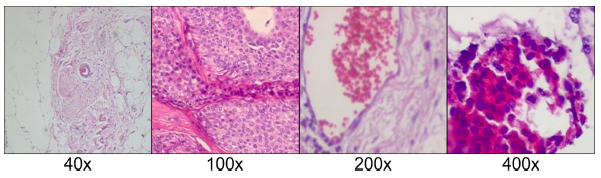
\includegraphics[scale=0.7]{figures/breast_histoimg_multiple_scales.png}}
	\caption{Example of histological images, captured at multiple magnification factors. Image from \cite{bayramoglu2016deep}}
	\label{histo_img}
\end{figure}

Due to the characteristics of these images, annotation in this field remains extremely expensive. Even a single sample requires many work hours from a trained expert, usually a doctor. Although not as costly as annotation, diagnosis also requires notable effort thus automating this process through the use of intelligent methods has the potential to streamline a process which affects millions of patients and non-patients. 

Fully automated systems in this field would allow people to get regular checks at a low price. This is essential in combating diseases like cancer in which early diagnosis drastically increases the survival rate. The promise of such models encouraged researchers to develop various datasets focused on different organs including the liver, prostate, colon and breasts.

One class of Deep Learning models which recently obtained impressive results in multiple histopathology Computer-aided Diagnosis problems are \textbf{Multitask (MT)} models. The benefits of the \textbf{Multitask Learning} \textbf{(MTL)} paradigm \cite{caruana1997multitask} are manifold. First of all, this type of approach usually results in algorithms with better generalization. Secondly, as a single sample may be used for two predictions, some components of the network, such as encoders, are able to exploit this increased data efficiency and achieve faster model convergence. Moreover, training a single Multitask network requires less computational resources when compared with the prospect of training two independent networks. 

All these desirable qualities make MT models well suited for intelligent applications in medicine, especially in Digital Histopathology where sample scarcity and massive image dimensions encourage the maximization of data efficiency and the reduction of the computational cost. 

\begin{figure}[htb]
    \centering
	\centerline{\includegraphics[scale=0.3]{figures/categories_mt_nets_v2.png}}
	\caption{Examples of Multitask network classes. Adapted from \cite{zhao2023multi}.}
	\label{mt_net_categ}
\end{figure}

The aim of this work is to analyse recent approaches from the Digital Histopathology field which employ Deep Multitask models, offer a taxonomy based on the choice of objectives and identify possible future research directions. This survey analyses those works which describe themselves as Deep Multi-Task Learning for the Histopathological Field. The papers which were considered were published and indexed by November 2023. For this review article, we used PRISMA principle to perform an objective search of publications investigating deep multi-task models applied in digital histopathology. The following key terms were used for searching in WOS and Scopus databases: “digital histopathology” AND “multi-task" AND ("Deep Learning" OR “Machine Learning").

Based on this literature we aim to answer the following research questions:
\begin{itemize}
  \item What is the current state of deep multi-task learning approaches in histopathology?
  \item What types of objectives were combined in order to increase performance in the field?
  \item What are the advantages, shortcoming and possible further research directions of the MTL paradigm in the field?
\end{itemize}

We aim to further improve this survey and extend the analyzed papers in order to encapsulate recent work from 2024 and beyond. We tried to showcase different ways of applying the multi-task learning paradigm in this field, thus the originality of the chosen objective were the main criteria in our selection. 

The rest of this work is structured in the following manner. In \textbf{Section \ref{chapter:RelatedWork}} Deep Multitask models are introduced. Next, \textbf{Section \ref{chapter:InvestigatedApproach}} analyses recent MT approaches applied in various histopathology problems. The advantages and limitations of the previously mentioned methods are discussed in \textbf{Section \ref{chapter:Discussion}}. Lastly, \textbf{Section \ref{chapter:5-Conclusions}} concludes the paper.

% An example of a floating figure using the graphicx package.
% Note that \label must occur AFTER (or within) \caption.
% For figures, \caption should occur after the \includegraphics.
% Note that IEEEtran v1.7 and later has special internal code that
% is designed to preserve the operation of \label within \caption
% even when the captionsoff option is in effect. However, because
% of issues like this, it may be the safest practice to put all your
% \label just after \caption rather than within \caption{}.
%
% Reminder: the "draftcls" or "draftclsnofoot", not "draft", class
% option should be used if it is desired that the figures are to be
% displayed while in draft mode.
%
%\begin{figure}[!t]
%\centering
%\includegraphics[width=2.5in]{myfigure}
% where an .eps filename suffix will be assumed under latex, 
% and a .pdf suffix will be assumed for pdflatex; or what has been declared
% via \DeclareGraphicsExtensions.
%\caption{Simulation results for the network.}
%\label{fig_sim}
%\end{figure}

% Note that the IEEE typically puts floats only at the top, even when this
% results in a large percentage of a column being occupied by floats.


% An example of a double column floating figure using two subfigures.
% (The subfig.sty package must be loaded for this to work.)
% The subfigure \label commands are set within each subfloat command,
% and the \label for the overall figure must come after \caption.
% \hfil is used as a separator to get equal spacing.
% Watch out that the combined width of all the subfigures on a 
% line do not exceed the text width or a line break will occur.
%
%\begin{figure*}[!t]
%\centering
%\subfloat[Case I]{\includegraphics[width=2.5in]{box}%
%\label{fig_first_case}}
%\hfil
%\subfloat[Case II]{\includegraphics[width=2.5in]{box}%
%\label{fig_second_case}}
%\caption{Simulation results for the network.}
%\label{fig_sim}
%\end{figure*}
%
% Note that often IEEE papers with subfigures do not employ subfigure
% captions (using the optional argument to \subfloat[]), but instead will
% reference/describe all of them (a), (b), etc., within the main caption.
% Be aware that for subfig.sty to generate the (a), (b), etc., subfigure
% labels, the optional argument to \subfloat must be present. If a
% subcaption is not desired, just leave its contents blank,
% e.g., \subfloat[].


% An example of a floating table. Note that, for IEEE style tables, the
% \caption command should come BEFORE the table and, given that table
% captions serve much like titles, are usually capitalized except for words
% such as a, an, and, as, at, but, by, for, in, nor, of, on, or, the, to
% and up, which are usually not capitalized unless they are the first or
% last word of the caption. Table text will default to \footnotesize as
% the IEEE normally uses this smaller font for tables.
% The \label must come after \caption as always.
%
%\begin{table}[!t]
%% increase table row spacing, adjust to taste
%\renewcommand{\arraystretch}{1.3}
% if using array.sty, it might be a good idea to tweak the value of
% \extrarowheight as needed to properly center the text within the cells
%\caption{An Example of a Table}
%\label{table_example}
%\centering
%% Some packages, such as MDW tools, offer better commands for making tables
%% than the plain LaTeX2e tabular which is used here.
%\begin{tabular}{|c||c|}
%\hline
%One & Two\\
%\hline
%Three & Four\\
%\hline
%\end{tabular}
%\end{table}


% Note that the IEEE does not put floats in the very first column
% - or typically anywhere on the first page for that matter. Also,
% in-text middle ("here") positioning is typically not used, but it
% is allowed and encouraged for Computer Society conferences (but
% not Computer Society journals). Most IEEE journals/conferences use
% top floats exclusively. 
% Note that, LaTeX2e, unlike IEEE journals/conferences, places
% footnotes above bottom floats. This can be corrected via the
% \fnbelowfloat command of the stfloats package.
\section{Background}
\label{chapter:RelatedWork}

Multitask models are network architectures created with the purposes of solving multiple, different, but related problems at the same time. This approach yielded impressive results in many Artificial Intelligence subfields such as: Computer Vision, Natural Language Processing and Reinforcement Learning as shown in \cite{crawshaw2020multi}.

Training a model using Multitask Learning can result in numerous benefits including faster inference and training, when compared to two or more separate networks; reduced overfitting and information optimization, as each sample becomes more valuable in a MTL environment. On the other hand, the disadvantage comes in the form of the increased complexity of finding symbiotic tasks. In some scenarios, stabilizing the MT network can become a cumbersome task. This is known in the literature as \textit{negative transfer}, a case in which learning valuable information in one task hinders the performance of other tasks encapsulated in the model.

Carefully choosing tasks and formulating them in a way which benefits each other is not an exact science, which follows certain protocols, at least yet. At the moment this combination is done based on intuition and through experimentation thus reducing the negative transfer can be seen as "the art" of building Multitask models. 

There are multiple works in the literature which showcase the unreasonable effectiveness of MT models, where multiple tasks "cooperate" to improve the performance in all problems tackled by the multi-headed network. Besides the increase in performance, MT has another interesting quality namely the fact that it more closely reflects human reasoning. The human learning process is almost never done in isolation, any new concept is learned through the prism of previous experiences and knowledge. Additionally, when learning multiple new concepts in the same time, the human mind usually attempts to find relationships between them. 

The combination of multiple tasks can be achieved through multiple categories of MT architectures identified in works such as \cite{crawshaw2020multi} and \cite{zhao2023multi}. The most prevalent are the following three: cascaded, normal (parallel) and cross-talk (interactive). A schematic illustration of these can be seen in \textbf{Figure \ref{mt_net_categ}}.

The most ubiquitous type of MT network is the parallel one. In this design, a common encoder extracts valuable features which are sent in multiple independent task specific modules. Depending on the relation between the approached tasks the individual modules can be further connected via one or multiple fusion blocks in  order to further increase performance, resulting in a interacted or cross-task MT model. A cascade network is obtained when the result of one task is used as an input or feature for the remaining tasks.

\begin{figure}[htb]
    \centering
	\centerline{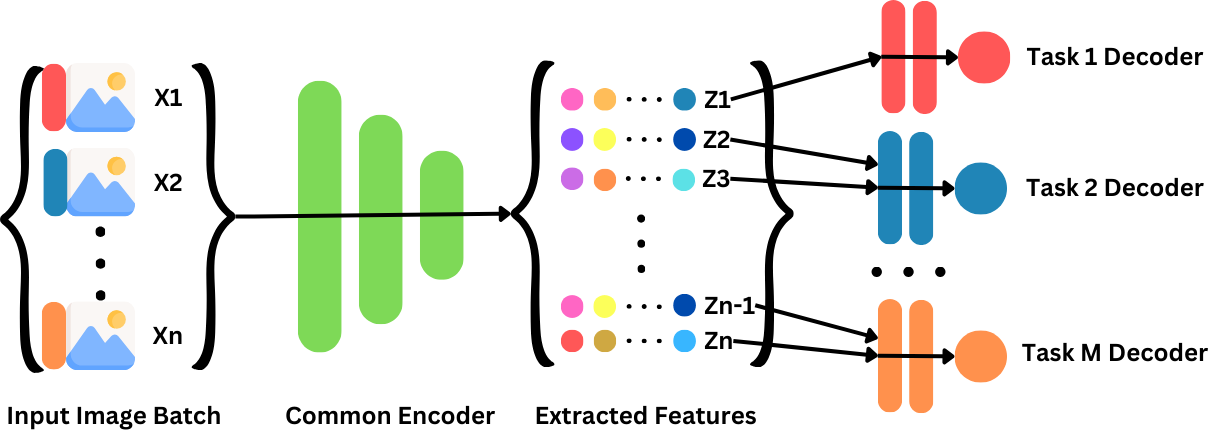
\includegraphics[scale=0.28]{figures/mt_pretraining_V2.png}}
	\caption{The proposed MT arhitecture for pre-training. Adapted from \cite{mormont2020multi}}
	\label{mt_pretaining}
\end{figure}

\begin{figure*}[htb]
    \centering
	\centerline{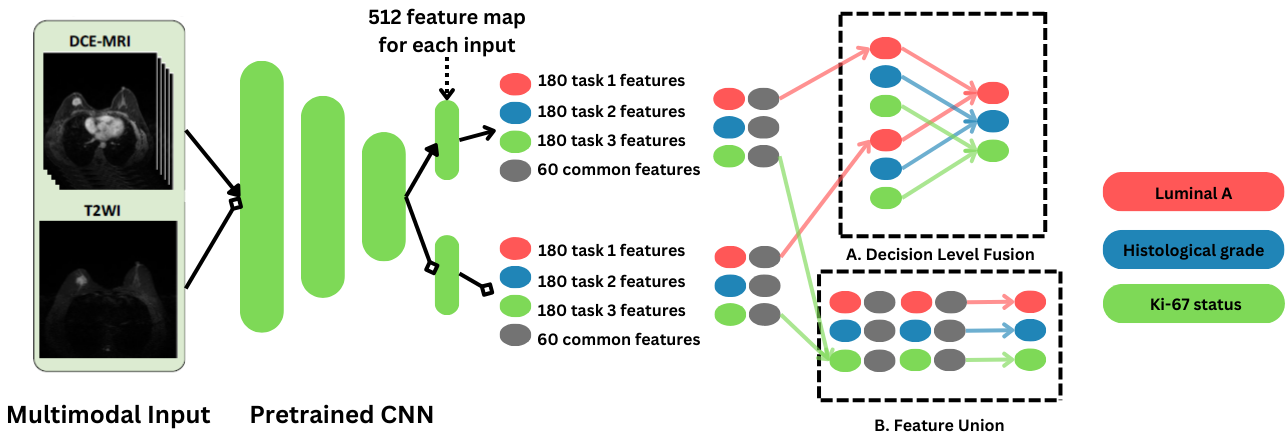
\includegraphics[scale=0.5]{figures/multimodal_multitask_V2.png}}
	\caption{Multi-modal Multitask architecture for Luminal A, Histological Grade and Ki-67 expression status classification. Image adapted from \cite{fan2022framework}}
	\label{multimodal_multitask}
\end{figure*}


Depending on the school of thought, some researchers argue that networks which process Multi-modal inputs are also included in the MT class of models. For this paper we will consider only approaches from the previously described three categories, although we will not disqualify multi-modal architectures as long as they are also part of said MT classes.

\begin{table}[]
    \caption{List of the datasets used by each analysed methods. Bolded names are used for sets which were used in multiple works. WSI denotes that the number of samples refers to full whole-slide images, otherwise the number represents the amount of patches. 
    }
    \label{table1}
    \centering
    \scalebox{0.88}{
    \begin{tabular}{|c|c|cr|}
    \hline
    \textbf{Method ref.}                                                & \textbf{Task}                    & \multicolumn{1}{c|}{\textbf{Dataset}}                                                                                                                                           & \textbf{No. Images}                                         \\ \hline
    \cite{bayramoglu2016deep}                    &                                  & { \textbf{BreaKHis \cite{spanhol2015dataset}}}                                                                                             & 7909                                                    \\ \cline{1-1} \cline{3-4} 
                                                                  &                                  & { \textbf{BreaKHis \cite{spanhol2015dataset}}}                                                                                             & 7909                                                    \\
                                                                  &                                  & \begin{tabular}[c]{@{}c@{}}Invasive Breast carcinoma \cite{dimitropoulos2017grading}\end{tabular}                                                            & 300                                                     \\ 
                                                                  % \cline{3-4} 
    \multirow{-3}{*}{\cite{li2020multi}}         &                                  & Janowczy Lymphoma \cite{janowczyk2016deep}                                                                                                                     & 374                                                    \\ \cline{1-1} \cline{3-4} 
    \cite{tan2022multi}                          &                                  & \begin{tabular}[c]{@{}c@{}}Zhejiang Cancer Hospital \\ (Private)\cite{tan2022multi}\end{tabular}                                                               & 954                                                     \\ \cline{1-1} \cline{3-4} 
                                                                  &                                  & Janowczyk6 \cite{janowczyk2016deep}                                                                                                                            & 277524                                                  \\
                                                                  &                                  & Janowczyk7 \cite{janowczyk2016deep}                                                                                                                            & 2244                                                    \\
                                                                  &                                  & Stroma LBP \cite{linder2012identification}                                                                                                                     & 2313                                                    \\
                                                                  &                                  & BACH18 Micro \cite{aresta2019bach}                                                                                                                             & 4800                                                    \\
                                                                  &                                  & { \textbf{UMCM Colorectal \cite{kather2016multi}}}                                                                                         & 5000                                                    \\
                                                                  &                                  & Necrosis \cite{mormont2018comparison}                                                                                                                          & 882                                                     \\ 
                                                                  % \cline{3-3}
                                                                  &                                  & ProliferativePattern \cite{mormont2018comparison}                                                                                                              & 1857                                                    \\
                                                                  &                                  & CellInclusion \cite{mormont2018comparison}                                                                                                                     & 3637                                                    \\
                                                                  &                                  & Lung \cite{mormont2018comparison}                                                                                                                              & 6331                                                    \\
                                                                  &                                  & Glomeruli \cite{maree2016approach}                                                                                                                             & 29213                                                   \\
                                                                  &                                  & Breast1 \cite{mormont2018comparison}                                                                                                                           & 23032                                                   \\
                                                                  &                                  & Breast2 \cite{mormont2018comparison}                                                                                                                           & 17523                                                   \\
                                                                  & \multirow{-18}{*}{\textbf{Cls.}} & Bone marrow \cite{maree2016approach}                                                                                                                           & 1291                                                    \\ \cline{2-4} 
                                                                  &                                  & Janowczyk1 \cite{janowczyk2016deep}                                                                                                                            & 31725                                                   \\
                                                                  &                                  & Janowczyk2 \cite{janowczyk2016deep}                                                                                                                            & 3402                                                    \\
                                                                  & \multirow{-3}{*}{\textbf{Seg}}   & { \textbf{Camelyon16 \cite{bejnordi2017diagnostic}}}                                                                                       & 292226                                                  \\ \cline{2-4} 
                                                                  &                                  & Janowczyk5 \cite{janowczyk2016deep}                                                                                                                            & 24870                                                   \\
                                                                  &                                  & MITOS-ATYPIA 14 \cite{roux2014mitos}                                                                                                                           & 64873                                                   \\
                                                                  &                                  & Warwick CRC \cite{sirinukunwattana2016locality}                                                                                                                & 2500                                                    \\
                                                                  &                                  & MouseLba \cite{mormont2018comparison}                                                                                                                          & 4284                                                    \\
                                                                  &                                  & HumanLba \cite{mormont2018comparison}                                                                                                                          & 5420                                                    \\
    \multirow{-22}{*}{\cite{mormont2020multi}}   &                                  & { \textbf{TUPAC2016 Mitosis \cite{veta2019predicting}}}                                                                                    & 77853                                                   \\ \cline{1-1}
    \cite{yu2021large}                           & \multirow{-7}{*}{\textbf{Det}}   & Gastric Cancer \cite{yu2021large}                                                                                                                              & 10315                                                   \\ \hline
                                                                  &                                  & CoNSeP \cite{graham2019hover}                                                                                                                                  & 41 WSI                                                  \\
    \multirow{-2}{*}{\cite{wang2021bend}}        &                                  & MoNuSegv1 \cite{kumar2017dataset}                                                                                                                              & 30 WSI                                                  \\ \cline{1-1}
    \cite{rezazadeh2023multi}                    &                                  & { \textbf{GlaS \cite{sirinukunwattana2017gland}}}                                                                                          & 165                                                     \\ \cline{1-1} \cline{3-4} 
                                                                  & \multirow{-4}{*}{\textbf{Seg}}   & { \textbf{Camelyon16 \cite{bejnordi2017diagnostic}}}                                                                                       & 292226                                                  \\ \cline{2-2}
    \multirow{-2}{*}{\cite{tellez2020extending}} & \textbf{Det}                     & { \textbf{TUPAC2016 Mitosis \cite{veta2019predicting}}}                                                                                    & 77853                                                   \\ \hline
    \cite{marik2022supervision}                  &                                  & { \textbf{UMCM Colorectal \cite{kather2016multi}}}                                                                                         & 5000                                                    \\ \cline{1-1} \cline{3-4} 
    \cite{tan2022multi}                          & \multirow{-2}{*}{\textbf{Cls}}   & \begin{tabular}[c]{@{}c@{}}Cancer Genome Atlas (TCGA) \cite{chen2020pathomic}\\  processed in \cite{mobadersany2018predicting}\end{tabular} & 1061                                                    \\ \hline
                                                                  &                                  & { \textbf{CRAG \cite{graham2019mild}}}                                                                                                     & 213                                                     \\
                                                                  &                                  & { \textbf{GlaS \cite{sirinukunwattana2017gland}}}                                                                                          & 165                                                     \\
    \multirow{-3}{*}{\cite{dabass2022mtu}}       & \multirow{-3}{*}{\textbf{Seg}}   & LC-25K \cite{borkowski2019lung}                                                                                                                                & 25000                                                   \\ \hline
                                                                  &                                  & { \textbf{CRAG \cite{graham2019mild}}}                                                                                                     & 213                                                     \\
                                                                  &                                  & { \textbf{GlaS \cite{sirinukunwattana2017gland}}}                                                                                          & {\color[HTML]{343434} 165}                              \\
                                                                  & \multirow{-3}{*}{\textbf{Seg}}   & Lizard \cite{graham2021lizard}                                                                                                                                 & 291                                                     \\ \cline{2-4} 
                                                                  &                                  & Kather100k \cite{kather2019predicting}                                                                                                                         & 100000                                                  \\
                                                                  &                                  & CRC-TP \cite{javed2020cellular}                                                                                                                                & 20 WSI                                                  \\
    \multirow{-6}{*}{\cite{graham2023one}}       & \multirow{-3}{*}{Cls}            & Internal colon biopsy \cite{wahab2022semantic}                                                                                                                  & 53362 \\ \hline
    \end{tabular}
    }
    \end{table}
    

In \cite{zhao2023multi}, a vast number of medical applications of Deep Multitask models are presented, briefly described and categorised based on their architecture and entity present in the input images. The authors showcase numerous approaches in which the MTL paradigm was used to improve performance in clinical practices which diagnose the following body areas and systems: brain, eyes, chest, cardiac, abdomen, musculoskeletal. Furthermore, they also offer a description of methods which processes histological images. 

\begin{figure*}[htb]
    \centering
	\centerline{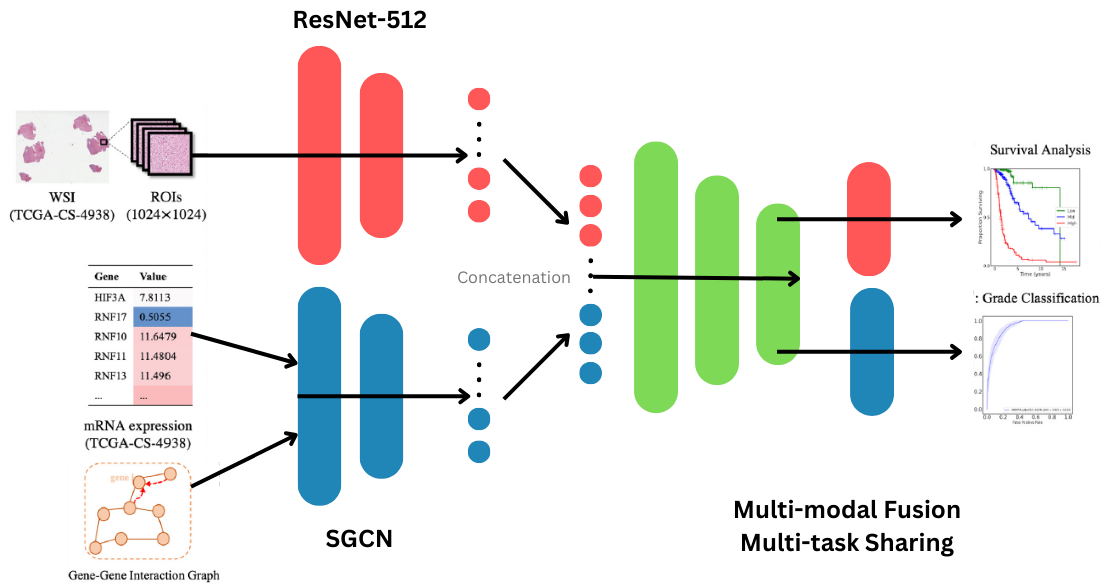
\includegraphics[scale=0.5]{figures/multimodal_multitask2_V2.png}}
	\caption{MultiCoFusion architecture from \cite{tan2022multi}}
	\label{multimodal_multitask2}
\end{figure*}

This paper differentiates itself from this impressive existing prior work through the following aspects:
\begin{itemize}
  \item The selection of approaches, which offer a larger, more focused view of Histopathology application 
  \item The perspective from which the analysis is conducted, as this paper will focus on the choice of tasks (i.e. classification +  segmentation), rather than the multi-task network class or the examined organ.
  \item The granularity of the analysis especially for the approaches considered to be the most representative.
\end{itemize}

\section{Deep Multitask Models for Histopathology}
\label{chapter:InvestigatedApproach}

We identified two different classes of MT approaches in the field of Histopathology when it comes to the types of combined learning procedures. The more common one comes in the form of an MT network which learns through two or more supervised objectives. In the other class of approaches, a supervised task is optimized simultaneously with an unsupervised one. The former is described in \textbf{Section \ref{hsmm}}, while \textbf{Section \ref{ssshmm}} presents the latter class of intelligent algorithms. Information regarding the datasets used by the presented methods can be found in \textbf{Table} \ref{table1}.

\subsection{Fully Supervised
Multitask Models}
\label{hsmm}

We classify approaches which combine multiple supervised tasks based on the nature of the combined objectives. Most MT networks perform two or more classifications in the same time. These types of approaches will be presented in \textbf{Subsection \ref{classification_mt}}. In \textbf{Subsection \ref{classification_reg_mt}} we present a technique which combines a classification objective with a regression problem. We continue by describing intelligent techniques which perform multiple segmentations simultaneously or a segmentation accompanied by another Image-to-Image inference in \textbf{Subsection \ref{segmentatiopn_mt}}. The last subsection from this section, \textbf{Subsection \ref{class_recog_mt}} analysis methods which fuse classification and any form of localization problems (segmentation or detection). 

\subsubsection{Multitask Classification Models}
\label{classification_mt}
A pioneering work from the field was introduced in \cite{bayramoglu2016deep}, where histological breast cancer images were classified as benign or malignant. This early MT approach can also predict the magnification factor. The resulting parallel architecture performs similarly to its single class equivalent showcasing that even early MT approaches allowed for the combination of multiple tasks without loss in performance. 


As Deep Learning matured, the performance of MT models continued to improve. Early approaches including the previous one evolved from simple binary-classification between benign and malignant tissue to fine-grained multi-class classification of the cancer cells as is the case with the intelligent algorithm proposed in \cite{li2020multi}. Furthermore, their proposed parallel MT network also predicts the severity of breast cancer through the other classification head which classifies the tissue's cancer grade. For the first objective, this method was able to achieve state-of-the-art results with a test accuracy of 93.43\%.

One limitation in the Digital Pathology space when compared with other areas in which AI showed impressive results is the lack of large, medical datasets which would allow \textbf{Transfer Learning (TL)}. Pre-training on ImageNet \cite{deng2009imagenet} allows networks to learn many valuable features for many other classification problems. The sheer size of it also made the dataset the choice even in the medical field, although it contains no medical image. In order to fill this gap in medical Computer-Vision, the authors of \cite{mormont2020multi} propose a MT approach able to aggregate the information from almost 90,000 images from 22 datasets. A common encoder is connected to 22 task-specific fully-connected layers, each tasked with classifying images from one of the datasets resulting in another parallel MT architecture. The learning objective is to reduce the mean loss obtained by averaging all the individual task-specific loss functions. A scheme of the model can be observed in \textbf{Figure \ref{mt_pretaining}}. The authors experimented with two established network backbones: ResNet50 \cite{he2016deep} and DenseNet121 \cite{huang2017densely}. The first one performs better and improves the results when compared to ImageNet pre-training in all scenarios. The most significant increase is achieved in bone marrow classification exceeding the pre-existing pre-training method by around 6\% accuracy.


Recently, researchers employed multi-modal data in tandem with MT architecture sin order to further develop the performance of existing approaches. One such approach was introduced in \cite{fan2022framework}. In this case, the multi-modality comes from the use of multi-parametric MRI images, a specific type of MRI which yields multiple types of medical data which better reflect the patient's state. The proposed network receives two inputs: the dynamic contrast-enhanced magnetic resonance images and T2-weighted images. Each has the benefit of better evidentiating complementary morphological characteristics of the human body. Starting from the ImageNet weights through the process of transfer learning, this MT network based on the VGG16 \cite{simonyan2014very} architecture learns to classify three cancer descriptors for breast cancer diagnosis: Luminal A, the histological grande and the Ki-67 expression. An illustration of the framework proposed in \cite{fan2022framework} is showcased in \textbf{Figure \ref{multimodal_multitask}}.




\begin{figure}[htb]
    \centering
	\centerline{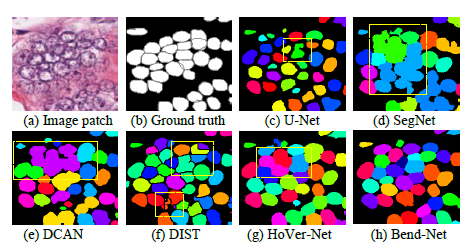
\includegraphics[scale=0.85]{figures/bend_results.png}}
	\caption{Inference examples of nuclei instance segmentation for multiple neural networks. Image from \cite{wang2021bend}}
	\label{bend_results}
\end{figure}


\begin{figure*}[htb]
    \centering
	\centerline{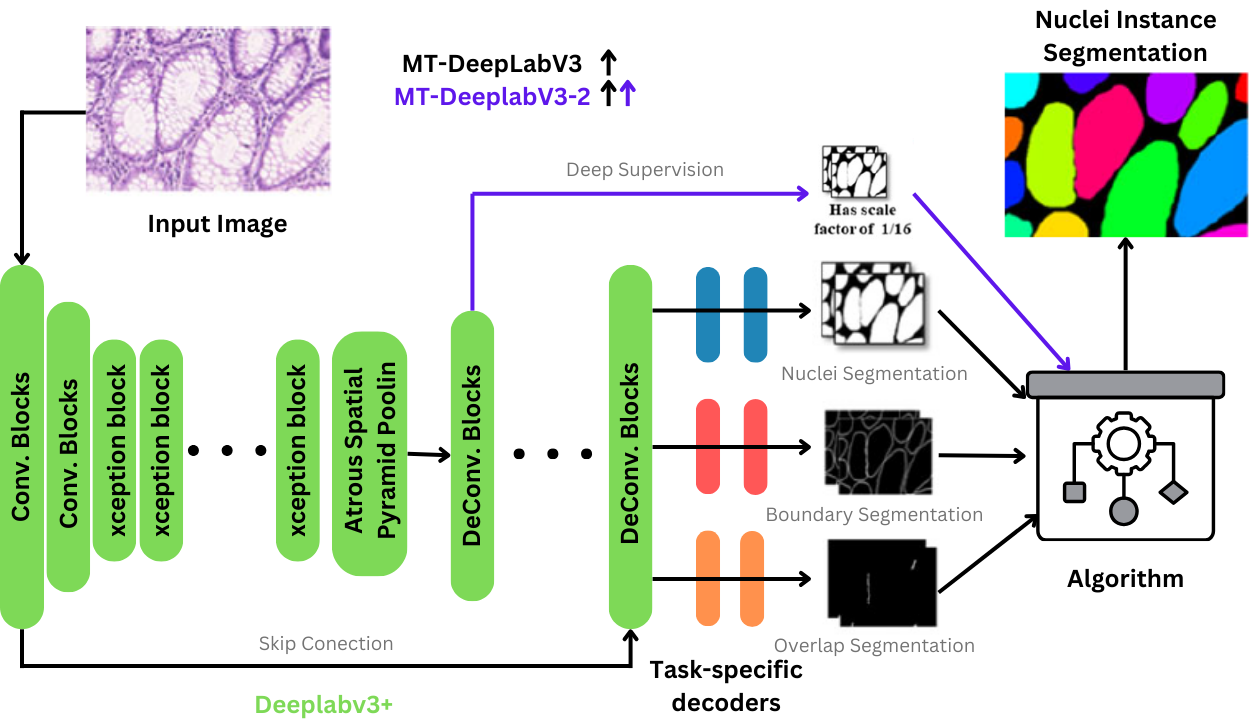
\includegraphics[scale=0.45]{figures/mt_deeplab_v2.png}}
	\caption{Scheme of MT-DeepLab and MT-DeepLab-2 architectures from \cite{rezazadeh2023multi}. The \textcolor{forestgreen}{green} components illustrate the original DeepLabV3. The black arrows show the Multi-Task DeepLab2, while the additional deeply-supervised objective represented with \textcolor{truepurple}{purple} is only present in the MT-DeepLab-2 version.}
	\label{mt_deeplab}
\end{figure*}

\subsubsection{Multitask Model for Classification and Regression}
\label{classification_reg_mt}
In \cite{tan2022multi}, the multi-modality is taken a step further as the input combines heterogeneous data: region of interests \textbf{(ROIs)} crops from a whole slide image \textbf{(WSI)} and a graph which represent the mRNA expression data. The model dubbed, Multitask
Correlation Learning \textbf{(MultiCoFusion)}, performs a classification task, in the form of cancer grade prediction in brain tissue and a regression task. The latter requires the network to predict the patient's survival risk. Unlike the previously described methods, MultiCoFusion does not have a single encoder. The multi-modality is processed through two different networks: ResNet152 for the histological images and a \textbf{Sparse Graph Neural Network (SGNN)} \cite{tan2021hierarchical} for the mRNA data. The extracted features are fused and passed to a MT module which extracts the most relevant features. Lastly, one prediction head is added for each task. Another unique aspect of this approach is the use of alternate learning instead of joint training, meaning that the network is updated based on only one objective for each batch. In this case, the determining objective is alternated after every batch.  An illustration of the proposed framework is showcased in \textbf{Figure \ref{multimodal_multitask2}}. MultiCoFusion is able to exceed all previous approaches, establishing itself as the state-of-the-art approach in both tasks.

\subsubsection{Multitask Segmentation Models}
\label{segmentatiopn_mt}

Another series of approaches combine two or more segmentation tasks in their MTL pipeline. Approaches \cite{wang2021bend} and \cite{rezazadeh2023multi} reformulate a single segmentation problem into a multi-objective one. The former approaches nuclei instance segmentation, while the latter tackles gland instance segmentation. In both problems, the entity instances overlap making a fine segmentation difficult resulting in a lower than desired performance. 

In both frameworks, the instance segmentation is transformed into three segmentation objectives. Besides the original segmentation task, the researchers add adjacent objective which facilitate the separation of overlapping instances. In \cite{wang2021bend}, a nuclei distance map and the overlapping segmentation are performed in order to guide the main task. In \cite{rezazadeh2023multi}, the second segmentation head performs contour segmentation, while the third is tasked with overlapped gland segmentation, in a similar manner with the previous approach. 

The approach from \cite{wang2021bend}, named Bend-Net has a U-Net \cite{ronneberger2015u} structure with three decoders and gets its name from the novel proposed bending loss function. This objective is also proposed to deal with wrongly segmented overlapped nuclei. This is achieved by finding convex and concave points and the retrieved structures. Concave points are drastically penalized as they suggest the wrong merge of two independent entities. The MT architecture combined with the bending loss outperforms numerous established networks in this task. Some results can be observed in \textbf{Figure \ref{bend_results}}

In \cite{rezazadeh2023multi}, the authors demonstrate the effective of their proposed MT approach over the original starting point networks (DeepLabV3+ \cite{chen2018encoder} and U-Net). Through the classic computer vision approach, starting from the instance segmentation ground-truth, they are able to obtain the contours segmentation map and the overlapping map, which in turn will be used as ground-truth in the MT pipeline. 

The resulting network which performs the three segmentation tasks is simply named MT-DeepLab. As a way to continue the improvement of this model in the second version of the architecture, MT-DeepLab-2, a forth segmentation task is added. The model is encouraged to learn the segmentation map as soon as possible through the addition of this forth objective which computes the instance segmentation loss at the start of the decoding path. Because the feature map has not yet gone through upsampling, this computation is done at a scale factor of 1/16. This type of learning is called Deep Supervision \cite{lee2015deeply}. The architecture is illustrated in \textbf{Figure \ref{mt_deeplab}}. Depending on the chosen metric either the first of the second MT-DeepLab outperforms all other networks which were considered for the task of gland segmentation.

\subsubsection{Multitask Models for Joint Classification and Recognition}
\label{class_recog_mt}

In \cite{yu2021large} a dataset for gastric cancer screening and localization is introduced. Furthermore, a MT network based on Deep Layer Aggregation is proposed \cite{yu2018deep}. Deformable convolutions \cite{dai2017deformable} are added to the model as many areas from WSIs contains little to no information, while other are densely packed with rich information. The method jointly learns to perform screening, a binary-classification problem in which tissue is classified as either normal or cancerous and semantic segmentation. The second task has the purpose of identifying the suspect areas in order to provide a justification for the diagnostic which could be verified by a doctor thus all cancerous cells have to be identified. 

The proposed network, to which we will refer to as \textbf{Multitask Deep Layer Aggregation (MT-DLA)} achieves state-of-the-art results when compared with existing segmentation networks outperforming all candidates when it comes to both the segmentation and screening objective. The only metric in which the model is outperformed is specificity, which is not as relevant when it comes to identifying dangerous diseases

Paper \cite{dabass2022mtu} includes another MT model which combines classification and segmentation, but unlike the previous approach it is applied for colon cancer. As many other networks which perform classification in a MTL environment in the field of Histopathology, the proposed network \textbf{Multitask U-Net (MTU)} classifies the tumour into either benign or malignant. Similar to the previous method, the segmentation is used to localize dangerous areas from the tissue. 

Besides the addition of these extra objective, MTU also employs attention modules \cite{vaswani2017attention}. Another defining characteristic of the approach is a novel block of layers design especially for WSIs, dubbed Hybrid Convolutional Learning Unit. This series of operations is a fusion between a Multi-Scalar Atrous Convolution, a Multi-Level Convolution and a Residual Block. The Multi-Scalar Dilated Transitional Unit is another newly introduced block which combines the results of four Atrous Convolutions with different dilation rates. The features are aggregated through a Global Average Pooling module. MTU was tested on two datasets, outperforming al competitor.

Similar to the work conducted in \cite{dabass2022mtu}, paper \cite{graham2023one} introduces a MT network for processing different types of entities: nuclei, glands, tissue and lumen. The proposed model, named Cerberus. employs a common encoder which feeds data to three parallel decoders tasked with segmentation (nuclei, glands, lumen) and a module forth parallel module for tissue type classification. This allows the encoder, a ResNet34, to learn rich features from multiple heterogeneous datasets, addressing data scarcity. U-Net like decoders are constructed for the segmentation tasks. The model achieves state-of-the-art-results exceeding the accuracy of other models in gland segmentation by almost 8\% and in lumen segmentation by 10\%. An overview of the framework is displayed in \textbf{Figure \ref{cerberus}}.


To further demonstrate the effectiveness of the encoder and their MTL strategy, the backbone is also used in two other transfer learning experiments. First of all, the pre-trained Cerberus encoder is used for the classification of nuclei. Next, the backbone is also employed in a detection task. Through the addition of object detection specific blocks which follow the RetinaNet \cite{lin2017focal} architecture, the model is able to learn to detect Signet ring cells. In nuclear classification, the pre-trained backbones yield a 4.6\% improvement on the test dataset when compared to previous approaches.

\begin{figure*}[htb]
    \centering
	\centerline{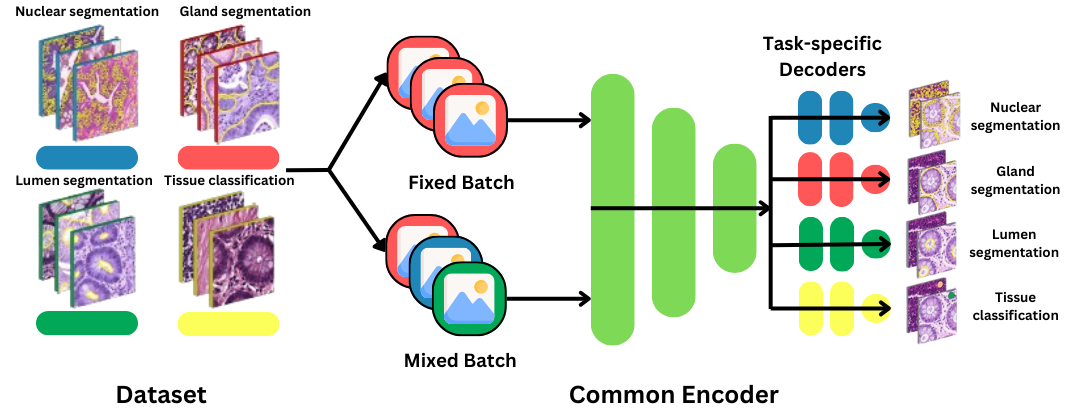
\includegraphics[scale=0.6]{figures/12_2_V3.png}}
	\caption{Cerberus \cite{graham2023one} framework overview.}
	\label{cerberus}
\end{figure*}

Lastly, the authors tackle the object subtyping. In this task, the segmented cell is further classified into four finer labels. As in the previous experiment the rest of the network is frozen, while the newly introduced decoder is taught to perform the multi-class segmentation. In all the experiments, Cerberus is shown to be a powerful network due to its encoder's ability to extract general, high-quality features.

\subsection{Supervised-Self-Supervised Hybrid Multitask Models}
\label{ssshmm}

In the previous subsection we have seen the effectiveness of MTL through the fusion of multiple supervised objectives. In practice, most medical datasets only provide labels for a single task thus being able to combine supervised with unsupervised objectives is a promising direction, which can enhance any single-task Deep Learning model. 

In \cite{tellez2020extending} the supervised classification objective is improved through the combination with Neural Image Compression \textbf{(NIC)}. The latter task, was introduced by the same authors in their previous work \cite{tellez2019neural}. NIC is a type of dimensionality reduction obtained through image reconstruction created specifically for medical Whole Slide Images. The symbiotic effect of this secondary unsupervised problem is proved in experiments which tackle two classification problems: Tumor Proliferation Assessment and  liver metastasis classification. For the second classification task, the MT approach exceeds the performance of its single-task counterpart by more than 8\% accuracy, resulting in state-of-the-art performance. 

The authors from \cite{marik2022supervision} also combine a supervised objective with an image reconstruction task. In this case, the supervised task comes in the form of colorectal cancer image similarity. The aim of their proposed framework is to obtained high quality features which could be used in classification tasks. In order to learn to compute image similarity, the triplet loss \cite{dong2018triplet} is used as as the objective function. Their proposed method is able to reach an accuracy of 95.22\% in the colorectal cancer histopathological \textbf{(CRCH)} dataset \cite{kather2016multi}, overcoming the best previous approach by around 2.5\% accuracy. 

Although this type of approach does not exploit information from another supervised objective, which could result in better performance it can be used to extend any existing single-task method as it does not require additional annotations.

\section{Discussion}
\label{chapter:Discussion}

Multitask learning approaches have numerous benefits, many being especially useful in the field of Digital Histopathology. Training strategies which allow the encoder to learn from multiple datasets address limitations posed by data scarcity. This yields an increase in performance when compared to single-task models. Moreover, even in setting in which the MTL paradigm is not used to this end, the fusion of two symbiotic objectives results in impressive performances. The MT architecture can also be used to boost the accuracy even when a single problem is tackled by reformulating the problem into multiple objectives. This showcases the versatility of this technique. Lastly, as multi-modal networks become more popular, MT networks establish themselves as a worthy candidate to process and extract information from heterogeneous data as prediction heads can be added for each data type as a way to complement the main objective. All these characteristics set MT models apart as an approach which can infer in a manner which is closer to human logic, having  potential in the explainability area as the field further matures. 

On the other hand, the MT Histopathology literature is still in early phases. Most models compare themselves against general architectures, which were not tailored for the approached medical task. The desire to solve multiple problems at the same time created a need for new datasets which contain annotations for all objectives. This is an extremely costly endeavour, which satisfied the requirements only in few cases. Even if multiple datasets exist in the field, combining them can prove to be cumbersome as the resulting super-set would have samples in which not all tasks have a ground-truth, as most databases only contain annotations for one or a few tasks. 

When it comes to the model themselves, the main limitation is the fact that almost all approaches follow the parallel MT architecture. Further experiments could be conducted in order to evaluate the possible improvements obtained through the transformation into a cross-talk or interactive approach. Vast studies could be conducted in order to search for effective fusion techniques between otherwise independent decoders, especially when two of the objectives are closely knit. 

Lastly, another underdeveloped niche which could prove to be a promising research direction consists of combining supervised objectives with more semi-supervised or even unsupervised ones. This would alleviate the need of costly annotation, even if the initial results have little chance of being comparable to the potential of two fully supervised ones. 


\section{Conclusions}
\label{chapter:5-Conclusions}

In conclusion, Multitask Learning is a powerful and versatile learning strategy, which can be exploited in order to create effective encoders applicable in numerous tasks. The valuable features mined by this intelligent approach can be used to obtain multiple relevant medical information through a single model pass, reducing training and inference time. This paradigm which lead to impressive performance in multiple tasks is still in early phases, at least in the medical image analysis area, leaving space for future research directions which could investigate relevant areas which were not yet covered by the existing literature. It is our firm belief that the current state of MT networks warrants further study especially when it comes to  cross-talk techniques and possible fusions between supervised and semi-supervised or unsupervised objectives.  

\balance

% trigger a \newpage just before the given reference
% number - used to balance the columns on the last page
% adjust value as needed - may need to be readjusted if
% the document is modified later
%\IEEEtriggeratref{8}
% The "triggered" command can be changed if desired:
%\IEEEtriggercmd{\enlargethispage{-5in}}

% references section

% can use a bibliography generated by BibTeX as a .bbl file
% BibTeX documentation can be easily obtained at:
% http://mirror.ctan.org/biblio/bibtex/contrib/doc/
% The IEEEtran BibTeX style support page is at:
% http://www.michaelshell.org/tex/ieeetran/bibtex/
%\bibliographystyle{IEEEtran}
% argument is your BibTeX string definitions and bibliography database(s)
%\bibliography{IEEEabrv,../bib/paper}
%
% <OR> manually copy in the resultant .bbl file
% set second argument of \begin to the number of references
% (used to reserve space for the reference number labels box)
% \bibliographystyle{plain}
\bibliographystyle{IEEEtran}
\bibliography{BibAll}






% that's all folks
\end{document}


